\section{Программа и методика испытаний}

В современном процессе разработки программных систем особое внимание уделяется качеству и надежности создаваемого продукта. Тестирование является неотъемлемой частью жизненного цикла программного обеспечения и направлено на выявление и устранение ошибок, обеспечение соответствия функционала заявленным требованиям, а также повышение общей устойчивости и безопасности системы. 

В рамках данной работы тестирование охватывает несколько ключевых направлений: проверка функционала, логгирование и мониторинг. Проверка функционала основывается на принципах \textit{GitOps} -- современного подхода к управлению инфраструктурой и приложениями с помощью систем контроля версий, что обеспечивает прозрачность, повторяемость и контроль изменений. Важной составляющей является организация тестовых окружений —- изолированных сред, в которых разворачиваются приложения и сервисы для детального анализа их поведения и выявления дефектов до попадания в продуктивную среду.

Концепция тестовых окружений предполагает создание среды, максимально приближенной к реальной, но независимой от основной системы. Это позволяет моделировать различные сценарии эксплуатации, проводить стресс-тесты и интеграционные проверки без риска воздействия на рабочих пользователей. Автоматизация развёртывания тестовых окружений с использованием инструментов \textit{Helm} и \textit{FluxCD} позволяет стандартизировать процесс, минимизировать человеческий фактор и быстро реагировать на изменения в кодовой базе и конфигурации.

Не менее важным аспектом является организация логгирования и мониторинга, которые обеспечивают непрерывный сбор информации о работе системы и позволяют оперативно обнаруживать и устранять неисправности. Использование современных инструментов, таких как \textit{Loki}, \textit{VictoriaMetrics}, \textit{Promtail} и \textit{Grafana}, обеспечивает комплексный подход к наблюдаемости и анализу производительности и стабильности приложений.

В совокупности описанные методы и инструменты создают комплексную программу тестирования и мониторинга, направленную на повышение качества продукта, снижение рисков и упрощение сопровождения. В данном разделе подробно рассмотрены возможности тестирования функционала, логгирования и мониторинга, а также описаны процессы создания и использования тестовых окружений, что позволяет обеспечить системный и эффективный подход к контролю качества разработанной системы.

Применение унифицированных инструментов в \textit{dev}- и \textit{prod}-средах обеспечивает воспроизводимость результатов и минимизирует вероятность ошибок, связанных с различиями в конфигурации. Дополнительно автоматизация процессов тестирования и сбора метрик позволяет оперативно выявлять регрессии и аномалии на ранних этапах жизненного цикла приложения.

\subsection{Применение нескольких сред развертывания}

В рамках проектируемой системы используются два полноценных и изолированных окружения: тестовое и продуктивное. Разделение позволяет проводить предварительную проверку всех изменений и обновлений в безопасной среде до их внедрения в рабочую эксплуатацию. Такая архитектура минимизирует риски сбоев и упрощает диагностику.

Каждое окружение развернуто в отдельном кластере \textit{Kubernetes}, имеющем собственные ресурсы, хранилища и средства мониторинга. Это обеспечивает полную независимость окружений и позволяет тестировать изменения в условиях, максимально приближенных к продуктивной среде.

Создание и обновление окружений автоматизировано с использованием инструментов \textit{Helm} и \textit{FluxCD}. Управление инфраструктурой осуществляется по принципам \textit{GitOps}, при котором все конфигурации хранятся в системе контроля версий. Изменения в репозиториях автоматически синхронизируются с кластером, обеспечивая повторяемость и прозрачность всех действий.

Тестовое окружение испольщуется для следующих задач:
\begin{itemize}
    \item предварительная проверка новых функциональных изменений;
    \item регрессионное тестирование при изменениих зависимостей;
    \item стресс-тестирование и проверка поведения системы при высоких нагрузках;
    \item верификация работы модулей логгирования и мониторинга.
\end{itemize}

С целью обеспечения изоляции и воспроизводимости, каждое развертывание в тестовом окружении выполняется в отдельном пространстве имён. Настройка осуществляется централизованно через шаблоны \textit{Helm}, с возможностью указания окружения через переменные.

Ниже представлена схема развёртывания тестового и продуктивного окружений (рисунок \ref{fig:environments-structure.png}).

\begin{figure}[ht]
    \centering
    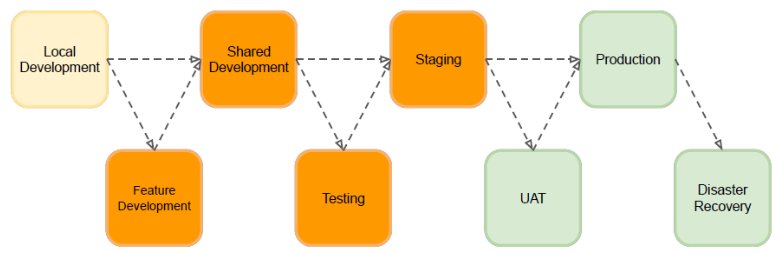
\includegraphics[width=0.9\linewidth]{\commonSecPathPrefix/../img/environments-structure.png}
    \caption{Архитектура развертывания тестового и продуктивного окружений}
    \label{fig:environments-structure.png}
\end{figure}

\subsubsection{Применение нескольких сред развертывания.}
В рамках разработки и эксплуатации системы реализовано использование нескольких изолированных сред: \textit{dev} и \textit{prod}. Каждая из них развернута в отдельном кластере \textit{Kubernetes}, что обеспечивает полную автономность окружений, изоляцию пользовательского и тестового трафика, а также безопасность выполнения операций.

Среда \textit{dev} предназначена для предварительного тестирования изменений. Все коммиты, поступающие в основную ветку репозитория, автоматически инициируют процесс обновления конфигурации в этом окружении. Это позволяет оперативно выявлять ошибки и дефекты в инфраструктуре, конфигурации или логике работы приложения до того, как они повлияют на конечных пользователей.

В среде \textit{prod} работают только проверенные и протестированные версии компонентов. Переход из \textit{dev} в \textit{prod} осуществляется вручную через pull-request в соответствующий репозиторий, где изменения проходят дополнительную проверку и одобрение. Таким образом, достигается контроль над процессом релизов и предотвращается неконтролируемое попадание нестабильного кода в продуктивную систему.

Для синхронизации конфигурации используется система \textit{FluxCD}, которая отслеживает изменения в репозиториях и автоматически приводит состояние кластера в соответствие с заданным описанием. Такой подход обеспечивает прозрачность, повторяемость и воспроизводимость изменений между средами.

Дополнительно для каждой среды применяются различные уровни мониторинга, логгирования и оповещений. Это позволяет на этапе разработки не только тестировать функциональность, но и контролировать метрики производительности, проверять настройки безопасности и обеспечивать полноту собираемых логов.


\subsection{Система автоматического отката изменений}

В процессе эксплуатации программных систем особенно важна возможность быстрого реагирования на непредвиденные ошибки и сбои, возникающие после внедрения новых версий приложений или конфигураций. Для обеспечения такой устойчивости используется система автоматического отката изменений (\textit{rollback}), которая позволяет вернуть систему в предыдущее стабильное состояние при обнаружении критических проблем.

В рамках данного проекта автоматический откат реализуется посредством интеграции с инструментами \textit{GitOps}, такими как \textit{FluxCD}, которые отслеживают состояние кластеров \textit{Kubernetes} и синхронизируют его с конфигурациями, хранящимися в репозитории. При возникновении отклонений или сбоев процесс отката может быть запущен автоматически или с минимальным вмешательством оператора.

Ключевые механизмы системы автоматического отката включают:

\begin{itemize}
    \item хранение версий конфигураций и манифестов в системе контроля версий \textit{Git}, что обеспечивает возможность точного восстановления предыдущего состояния;
    \item использование \textit{Helm} для управления релизами и упрощения процессов обновления и отката приложений;
    \item мониторинг состояния приложений с помощью системы наблюдаемости, что позволяет своевременно обнаруживать ошибки, инициирующие откат;
    \item настройка правил автоматического отката, которые могут базироваться на метриках доступности, времени отклика, частоте ошибок и других параметрах.
\end{itemize}

Таким образом, система автоматического отката обеспечивает высокий уровень надежности и минимизирует время простоя сервисов, снижая риски, связанные с обновлениями и изменениями в инфраструктуре и приложениях.



\subsection{Организация сбора метрик}

Сбор и анализ метрик является важнейшей частью обеспечения наблюдаемости и стабильности программных систем. В рамках данного проекта организация сбора метрик построена на использовании системы \textit{VictoriaMetrics}, которая позволяет эффективно агрегировать, хранить и обрабатывать большие объемы временных рядов данных.

Метрики собираются с различных уровней инфраструктуры и приложений:

\begin{itemize}
    \item системные метрики: загрузка процессора, использование памяти, состояние сети и дисков;
    \item бизнес-метрики: количество обработанных запросов, время ответа, уровень ошибок;
    \item пользовательские метрики: параметры, специфичные для бизнес-логики и пользовательского взаимодействия.
\end{itemize}

Для сбора данных используется \textit{Prometheus}-совместимый интерфейс, а для их передачи применяется агент \textit{Promtail}, который собирает логи и метрики, отправляя их в \textit{VictoriaMetrics} и \textit{Loki} для централизованного хранения и последующего анализа.

Основные преимущества используемой архитектуры сбора метрик:

\begin{itemize}
    \item высокая производительность и масштабируемость системы хранения метрик;
    \item поддержка долгосрочного хранения данных с настройками ретеншн и агрегации;
    \item возможность построения дашбордов и визуализации данных с помощью \textit{Grafana};
    \item интеграция с системой оповещений для своевременного информирования о проблемах.
\end{itemize}

Метрики включают данные о нагрузке на \textit{CPU}, использовании памяти, сетевом трафике, а также специфичные бизнес-метрики, позволяющие отслеживать качество работы приложений. Мониторинг настроен на сбор данных с различной степенью детализации и периодичностью, что позволяет выявлять аномалии и оптимизировать работу системы. Пример дашборда мониторинга представлен на рисунке \ref{fig:metrics_collection_dashboard}.
\begin{figure}[ht]
    \centering
    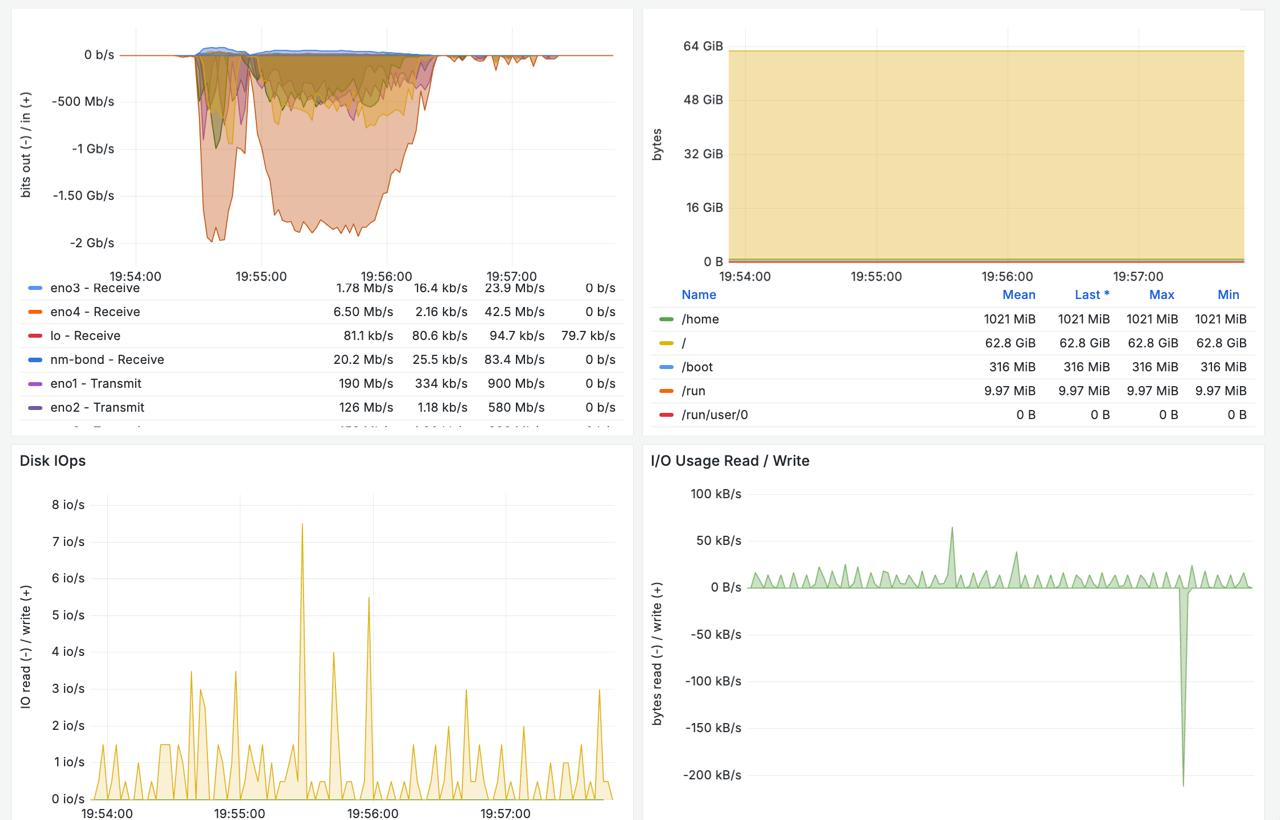
\includegraphics[width=0.8\linewidth]{\commonSecPathPrefix/../img/metrics_collection_dashboard.png}
    \caption{Пример дашборда мониторинга метрик в \textit{Grafana}}
    \label{fig:metrics_collection_dashboard}
\end{figure}

Реализованная система сбора метрик позволяет проводить как оперативный мониторинг, так и детальный анализ исторических данных, что способствует быстрому выявлению и устранению неисправностей, а также оптимизации работы программного обеспечения и инфраструктуры.


\subsection{Работа системы реагирования на аномалии}

Система реагирования на аномалии является ключевым элементом обеспечения устойчивости и надежности программной системы. Её задача -- своевременно обнаруживать отклонения в поведении приложений и инфраструктуры, которые могут свидетельствовать о сбоях, ошибках или потенциальных угрозах.

В рамках проекта реализован комплексный подход к обнаружению аномалий, включающий следующие компоненты:

\begin{itemize}
    \item сбор метрик и логов в режиме реального времени с использованием \textit{VictoriaMetrics} и \textit{Loki};
    \item настройка правил оповещений в \textit{Alertmanager} на основе заранее определённых пороговых значений для ключевых показателей производительности и стабильности;
    \item использование эвристических алгоритмов и анализ временных рядов для выявления нетипичного поведения, выходящего за пределы установленных норм;
    \item интеграция с системой уведомлений, позволяющая оперативно информировать ответственных сотрудников о возникших инцидентах через различные каналы (\textit{email}, мессенджеры и др.);
    \item периодический анализ инцидентов с целью уточнения и корректировки правил оповещений, минимизации ложных срабатываний и повышения точности обнаружения реальных проблем.
\end{itemize}

Такой подход обеспечивает непрерывный мониторинг состояния системы и позволяет быстро реагировать на возникающие проблемы, снижая время простоя и минимизируя негативное влияние на пользователей и бизнес-процессы. Важной частью системы реагирования является возможность автоматизации некоторых действий по устранению инцидентов, что в перспективе позволит перейти к более продвинутому уровню самовосстановления инфраструктуры.

\subsection{Анализ журнала сообщений}

Анализ журнала сообщений (логов) играет важнейшую роль в диагностике и устранении неисправностей, а также в обеспечении безопасности и аудита системы. Логирование позволяет получать детальную информацию о работе компонентов, пользовательских действиях и внутренних событиях.

В нашей системе для централизованного сбора и хранения логов используется стек \textit{Loki} с \textit{Promtail} на стороне агентов, который обеспечивает эффективное агрегирование и индексирование логов. Для визуализации и анализа применяются панели \textit{Grafana} с продвинутыми возможностями фильтрации, построения запросов и настройки оповещений.

Основные возможности анализа журналов включают:

\begin{itemize}
    \item структурированный поиск по ключевым словам и меткам, позволяющий быстро находить нужные записи;
    \item агрегация и группировка по временным интервалам для выявления паттернов и повторяющихся ошибок;
    \item построение графиков и дашбордов для визуального мониторинга тенденций и аномалий;
    \item интеграция с системой оповещений для своевременного уведомления о критических событиях;
    \item возможность настройки ротации и хранения логов с учетом требований к сохранности и объему данных.
\end{itemize}


Гибкий язык запросов позволяет быстро находить необходимые записи, что значительно упрощает процесс отладки и расследования инцидентов. Пример выполнения запроса и результатов поиска в системе логирования приведён на рисунке \ref{fig:loki_log_query}.

\begin{figure}[ht]
    \centering
    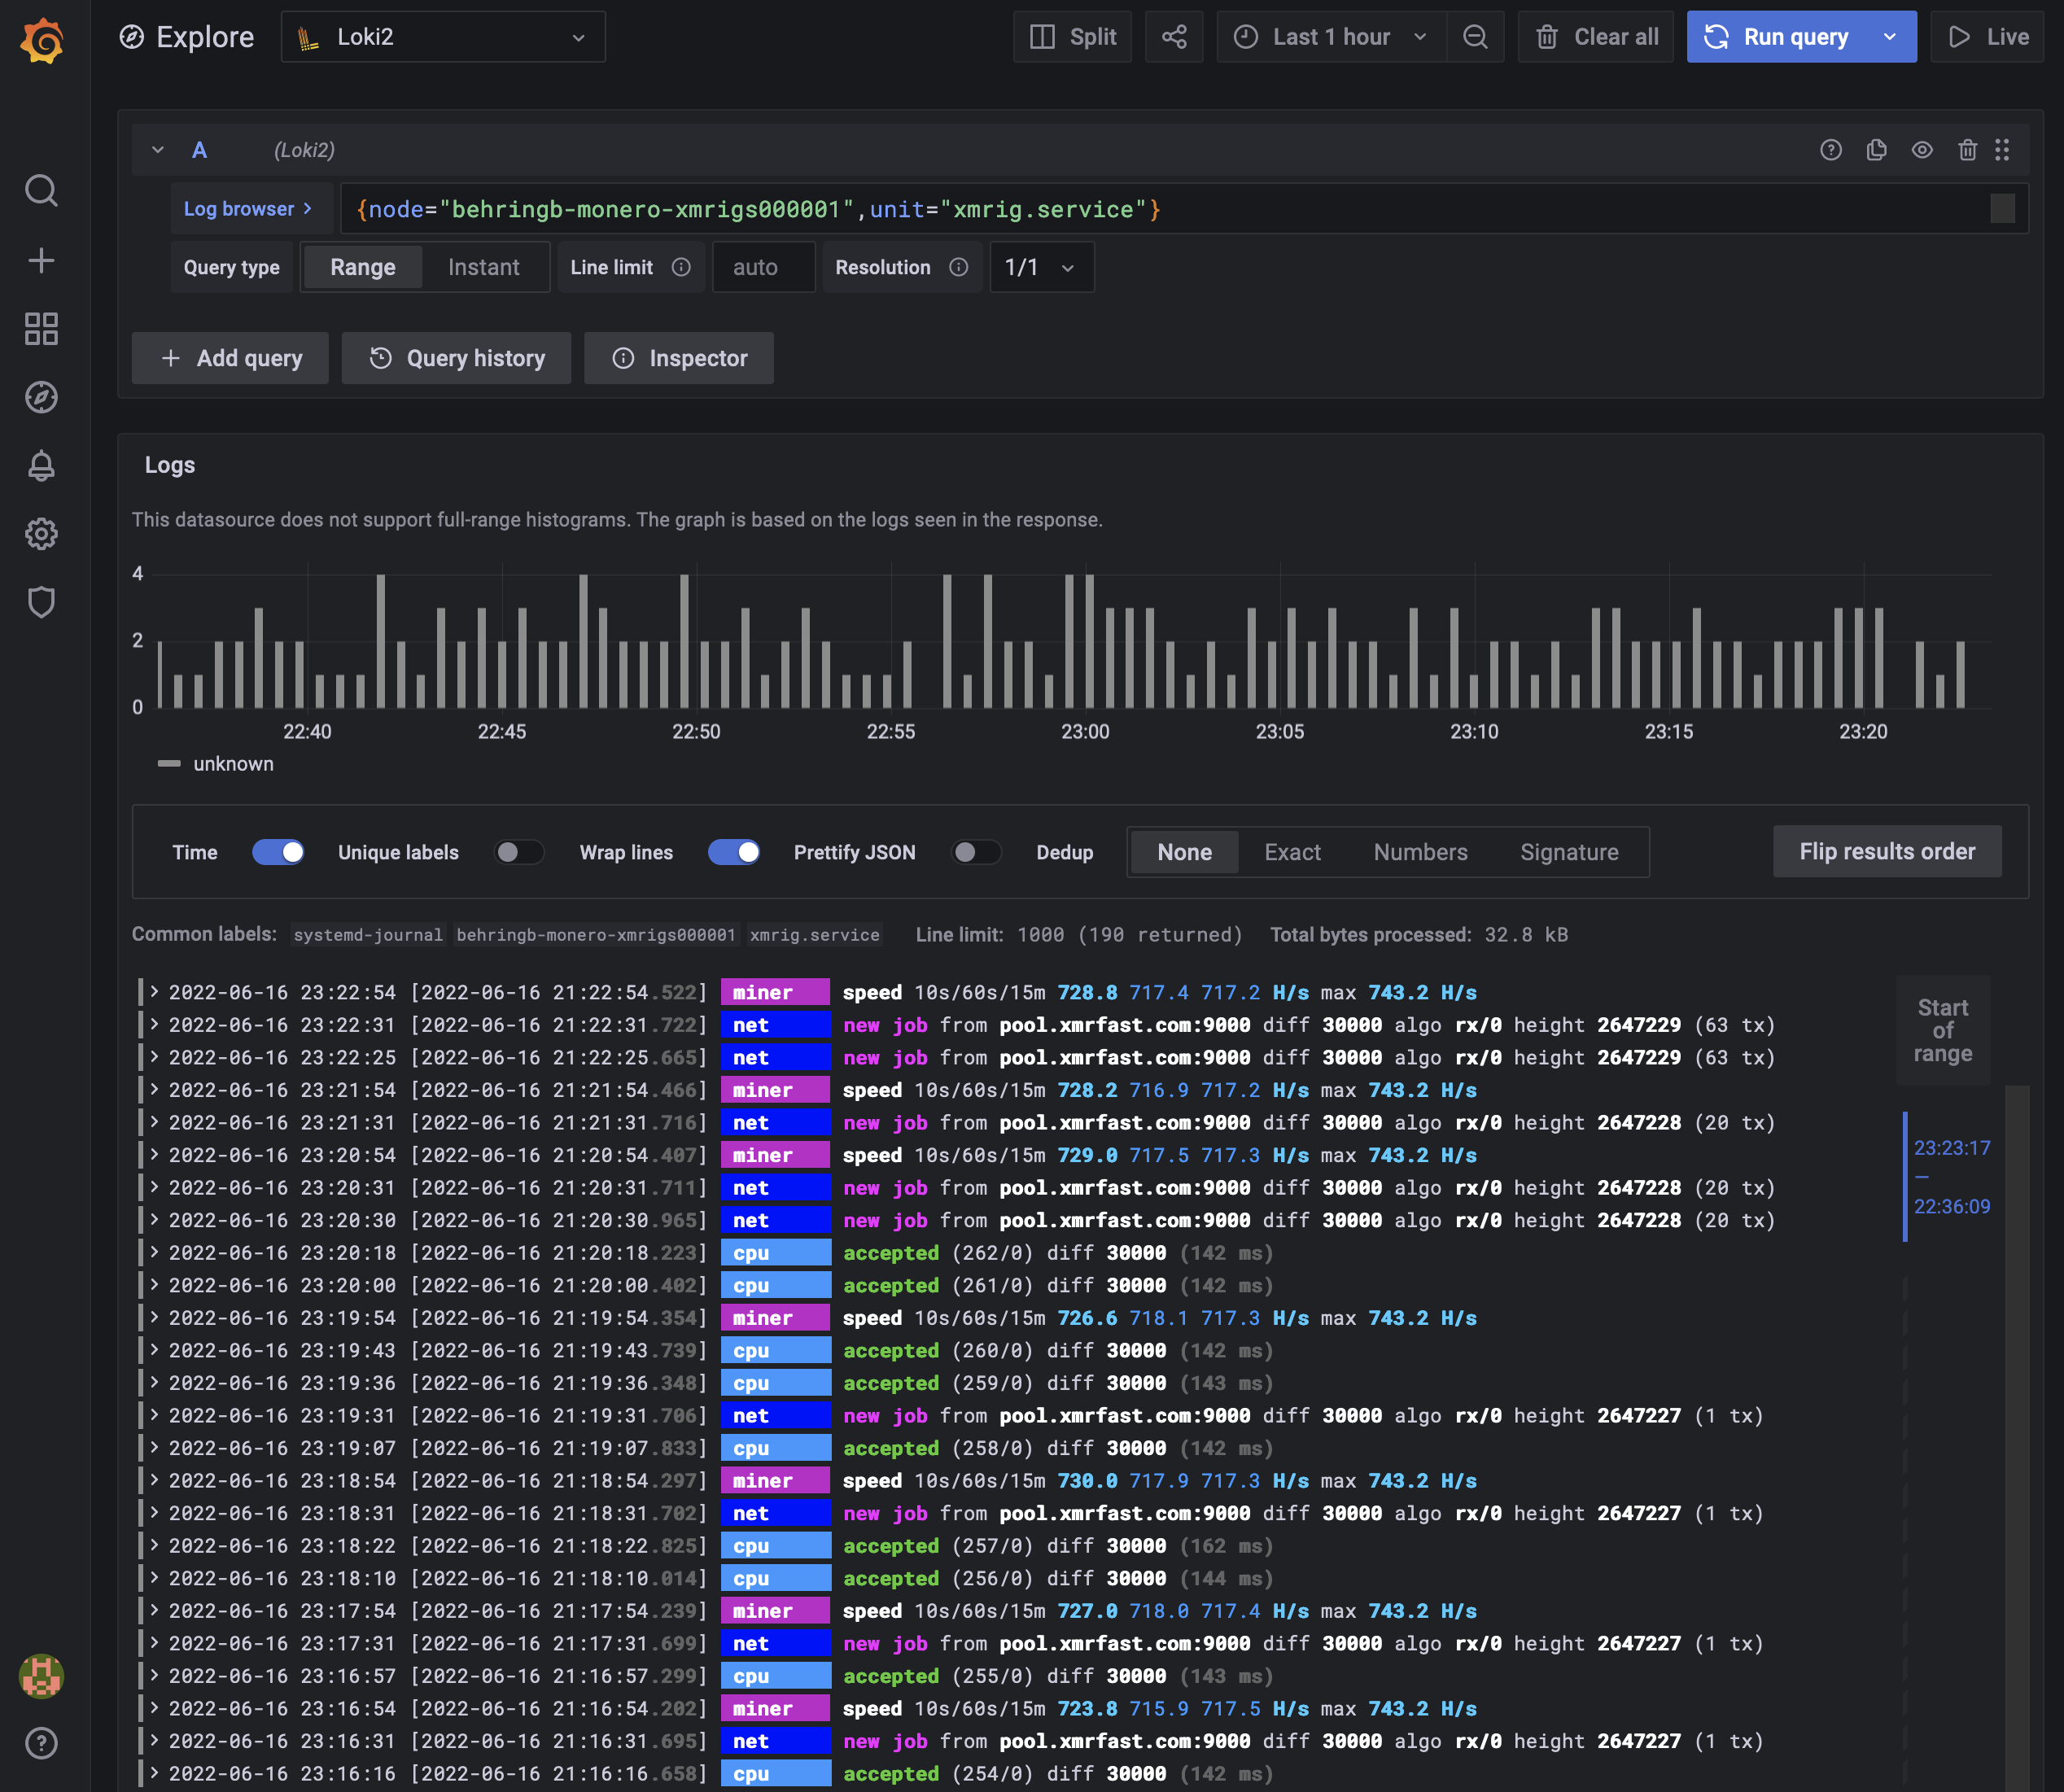
\includegraphics[width=0.8\linewidth]{\commonSecPathPrefix/../img/loki_log_query.png}
    \caption{Пример запроса и результатов поиска в системе \textit{Loki}}
    \label{fig:loki_log_query}
\end{figure}

Проведение регулярного анализа журналов позволяет не только оперативно выявлять и устранять проблемы, но и проводить ретроспективный аудит, выявлять узкие места в системе, а также оптимизировать производительность и безопасность.

